\documentclass[a4paper,14pt]{article}
\usepackage[T1]{fontenc}
\usepackage[utf8]{inputenc}
\usepackage[russian]{babel}
\usepackage[14pt]{extsizes}

%\usepackage{pscyr}
\usepackage{cmap}
\usepackage{indentfirst}
\usepackage{autonum}
\usepackage{amsfonts}
\usepackage{amsmath}
\usepackage{amssymb}
\usepackage{amsthm}
\usepackage{upgreek}
\usepackage{graphicx}
\usepackage{listings}
\usepackage{multirow}
\usepackage{dsfont}
\usepackage{setspace,amsmath}

\usepackage[unicode, pdftex]{hyperref}
\usepackage[left=30mm, top=20mm, right=15mm, bottom=20mm, footskip=10mm]{geometry}

\begin{document}
	\selectlanguage{russian}
	\setcounter{page}{0}
	
	\begin{center}
		\small{Министерство науки и высшего образования Российской Федерации}\\
		\small{Федеральное государственное бюджетное образовательное учреждение}\\
		\small{Высшего образования}\\
		\small{\textbf{«Северо-Осетинский государственный университет\\
				имени Коста Левановича Хетагурова»}}\\
		
		\hfill \break
		\hfill \break
		\hfill \break
		\hfill \break
		\hfill \break
		\hfill \break
		\hfill \break
		\hfill \break
		\hfill \break
		
		\normalsize{Дипломная работа}\\
		\large{\textbf{Seq2seq подход для задач Машинного Перевода}}\\
		
		\hfill \break
		\hfill \break
		\hfill \break
		\hfill \break
		\hfill \break
		\hfill\break
	\end{center}
	
	\begin{flushright}
		\textbf{Выполнил:}\\
		Студент 4 курса направления:\\
		«Прикладная математика и информатика»\\
		\textit{Гамосов Cтанислав Станиславович \underline{\hspace{3cm}}}\\
	\end{flushright}
	
	\hfill
	
	\begin{flushright}
		\textbf{Научный руководитель:}\\
		Кандидат физико-математических наук:\\
		\textit{Басаева Елена Казбековна \underline{\hspace{3cm}}}\\
	\end{flushright}
	
	\hfill
	
	\begin{flushright}
		\textbf{Консультант}\\
		Старший преподаватель: \\
		\textit{Макаренко Мария Дмитриевна \underline{\hspace{3cm}}}\\
	\end{flushright}
	
	\normalsize{ \hspace{28pt}} \hfill \break
	\begin{center} Владикавказ 2022 \end{center}
	
	\thispagestyle{empty}
	\tableofcontents
	\thispagestyle{empty}
	\clearpage
	\newtheorem{theorem}{Теорема}
	
	\section{Введение}
	
	\textbf{Seq2seq} - это семейство подходов машинного обучения, используемых для обработки естественного языка. Основные задачи для которого используется данные методы: нейронный перевод, субтитры к изображениям, разговорные модели и обобщение текста.
	
	Первоначальный алгоритм, который в процессе породил целое семейство методов, был разработан \textit{Google} для использования в машинном переводе. Как уже можно заметить за последнюю пару лет коммерческие системы стали удивительно хороши в  переводе - посмотрите, например, \textit{Google Translate}, \textit{Яндекс}-переводчик, переводчик \textit{DeepL}, переводчик \textit{Bing Microsoft}.
	
	Так же \textbf{seq2seq} технология несет в себе огромный потанцевал, помимо привычного машинного перевода между естественными языками, вполне реализуем перевод между языками программирования (\textit{Facebook AI "Глубокое обучение переводу между языками программирования"}). Поэтому возможности применений такого рода подходов довольно велики. В связи с этим под машинным переводом будет подразумеваться любая задача \textbf{seq2seq}, если точнее, то перевод между последовательностями любой природы.
	
	\clearpage
	
	\section{Формализация задачи машинного перевода}
	Формально в задаче машинного перевода у нас есть входная последовательность $x_{1}, x_{2}, ... x_{m}$ и последовательность вывода $y_{1}, y_{2}, ... y_{n}$, само собой длинна данных последовательностей может отличатся. Саму процедуру \textit{перевода} можно рассматривать как нахождение искомой последовательности, которая является наиболее вероятной с учетом входных данных. Формально искомая последовательность, которая максимизирует условную вероятность $p(y|x): y^{'} = argmax[p(y|x)]$.
	
	Когда человеку известны уже два языка с которыми он работает, то уже при переводе можно сказать насколько хорошо справилась модель, является ли перевод естественным и насколько он приятен на слух. Однако такой вид анализа неприемлем для машины, поэтому нам стоит проанализировать уже имеющуюся функцию $p(y|x,\theta)$ с неким параметром $\theta$, а затем найти его $argmax$ для $y^{'} = argmax_{y}[p(y|x, \theta)]$.
	
	Прежде чем перейти к самой задачи перевода, нужно ответить на 3 вопроса:
	
	\begin{itemize}
		\item \textbf{Моделирование}: Как работает модель для $p(y|x, \theta)$?
		\item \textbf{Обучение}: Как найти параметр $\theta$?
		\item \textbf{Вывод}: Как понять, что текущий $y$ лучший?
	\end{itemize}
	
	\clearpage
	
	\section{Задача машинного перевода}
	
	$source = (x_1, x_2, ... , x_n)$ - The cat sits on the floor
	
	$target = (y_1, y_2, ... , y_m)$ - Кошка сидит на полу
	
	Основная задача машинного перевода - найти наиболее вероятную последовательность для $target$ языка при условии, того что входная последовательность будет на $source$ языке.
	
	$target^{'} = argmax_{target} P(target | source, \theta)$
	
	$P(target | source) = P(y_1, y_2, ... , y_3 | source) = \\
	= P(y_1 | source) \dot P(y_2 | y_1, source) ... P(y_m | y_1, ... ,y_{m - 1}, source)$
	
	На самом деле модель машинного перевода это ничто иное как обычная языковая модель, но она является ограниченной за счет наличия ($source$)
	
	Так и есть ведь наша модель должна генерировать не просто текст, как это делают обычные языковые модели, а текс с некими ограничениями. Если точнее то необходимо генерировать текст, который будет являться переводом нашей входной последовательности с какого-то языка
	
	\textbf{Решение задачи машинного перевода}
	
	Правиловые системы
	
	Статистические системы
	
	Нейронные модели
	 
	\clearpage
	
	\section{Структура Encoder-Decoder}
	
	Наиболее распространенная модель \textbf{Sequence-to-sequence (seq2seq}) являются модель \textbf{Encoder-Decoder}, в которой обычно используют \textbf{рекуррентную нейронную сеть} (\textbf{RNN}) для кодирования исходной последовательности в один вектор.
	
	На самом деле полученный вектор можно представить как набор образов сущностей с образами взаимоотношений между ними. Этот вектор затем декодируется вторым \textbf{RNN}, который учится выводить выходное предложение, генерируя его по одному слову за раз.
	
	\begin{figure}[htbp]
		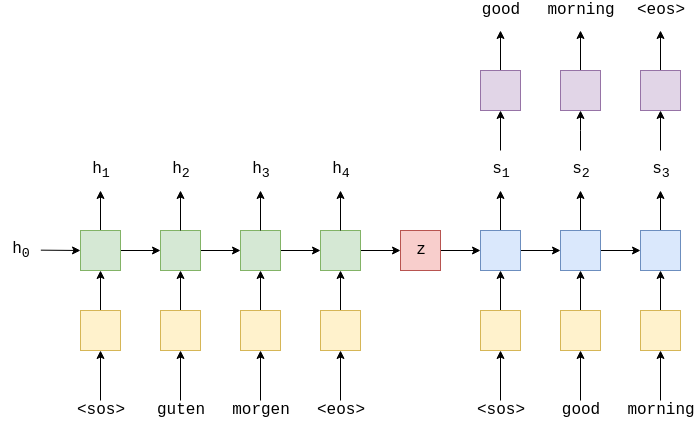
\includegraphics[width=\linewidth]{img/encoder-decoder-img-1.png}
	\end{figure}
\end{document}